\chapter{Machine Learning \ac{PSD}}
\label{chapter:ML-PSD}
4
Two algorithms will be investigated: first a \ac{VAE} and secondly a \ac{SOM}

\section{Data cleaning}
\label{sec:data-cleaning}
Raw charge waveforms\footnote{For \textit{raw} we mean waveforms already processed with LEGEND dedicated software, but still not selected in terms of energy, \ac{PSD} parameters or other features, as introduced at the end of Sec. \ref{subsubsec:data-structureL200}.} are not suitable for any machine learningg algorithm implementation as they are very different between one another under multiple aspects. In order to cope with this problem, a series of selection and cleaning procedures have been applied to them obtaining, at the end of said process, current waveforms in the energy range of interest.

The first data processing step that has been applied to raw waveforms is an energy-based cut around the region of interest, specifically encircling the \ac{DEP} of ${}^{208}$Tl and the \ac{FEP} of ${}^{212}$Bi. Hence, only data between 1550 keV and 1650 keV from the whole considered dataset have been saved, discarding all the other. This is for sure a choice based on the work purposes, but also a computational needing in order to neglect data that would be unused from the very beginning. Recalling Fig. \ref{fig:TlBi-spectrum} the energy cut is depicted in Fig. \ref{fig:cut_region} for run \textit{r000} of period \textit{p03}. Moreover data have been filtered with boolean masks provided together with raw data; said filters are needed to discard useless events. Particularly the filters that have been considered are listed in Tab. \ref{tab:quality_cuts}.

\begin{figure}[H]
    \centering
    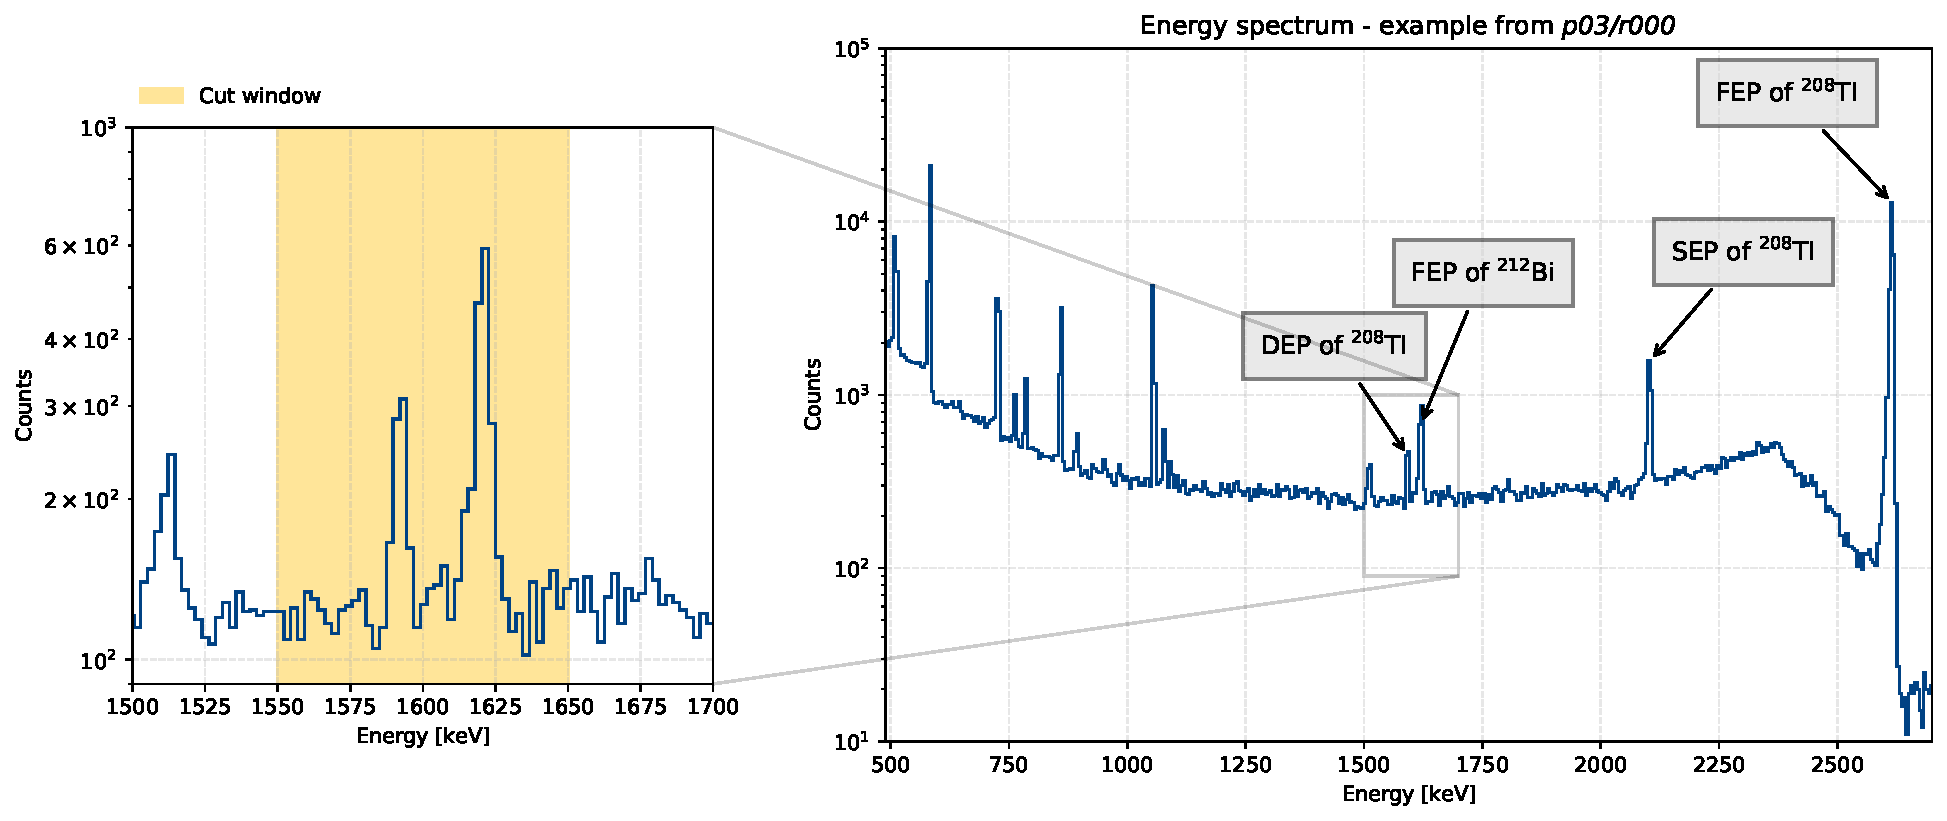
\includegraphics[width=\textwidth]{plots/energy_spectrum-cut_window.pdf}
    \caption{Example of the energy spectrum recorded in the calibration from \textit{p03/r000}. The energy region of the cut is highlighted.}
    \label{fig:cut_region}
\end{figure}

\begin{table}[H]
    \centering
    \renewcommand{\arraystretch}{1.2} % Migliora la spaziatura verticale delle righe
    \begin{tabular}{@{} l p{10cm} @{}}
        \toprule
        \textbf{Quality Cut} & \textbf{Discard (Events filtered)} \\
        \midrule
        discharge & discharges \\
        saturated & saturated waveforms (typically from muons) \\
        baseline pile-up & events caused by high-rate overlapping in the baseline \\
        tail pile-up & events caused by high-rate overlapping in the tail \\
        valid baseline & events with noise or discontinuities in the baseline \\
        valid tail & events with noise or discontinuities in the tail \\
        valid positive leading edge & events with noise bursts in the rising edge of the waveform \\
        valid CUSP minimum energy & events dominated by electronic noise at low energies \\
        valid drift time & events with a very high drift time \\
        \bottomrule
    \end{tabular}
    \caption{Summary of Quality Cuts and discarded events.}
    \label{tab:quality_cuts}
\end{table}

As soon as the energy cut and the event cut are performed, waveforms need to pass through a series of processes in order to obtain suitable inputs algorithms to be implemented. 
Firstly the mean value of the baseline is computed from the first 300 points of the raw charge waveform expressed in ADC counts and it is subtracted from all of the other points. Subsequently the baseline-subtracted charge waveform is normalised in order to have all of the waveforms with values between 0 and 1. After that, current waveforms are obtained from charge ones via time derivation using $dt = 16 ns$ that arises from the sampling rate of 62.5 MHz. Current waveforms are then filtered using a butterworth filter designed to remove high frequency parts of the signal mainly affecting the baseline part. Lastly, waveforms are aligned with respect to the first peak of the current signal and trimmed around the alignement point with 100 samples before it and 100 after it. 
Once all of these steps are completed, what we obtain is a suitable input for the \ac{VAE} model that is to be implemented as will be described in Sec. \ref{sec:model-implementation}. An example of the process is shown in Fig. \ref{fig:data-cleaning}, highlighting the two typical behaviours of \ac{SSE} waveforms (in red) and \ac{MSE} ones (in blue). %; examples of the other periods and runs can be found in the related Appendix \ref{app:waveforms}.

\begin{figure}[H]
    \centering
    
    % --- Prima figura (a) ---
    \begin{subfigure}[H]{0.48\textwidth}
        \centering
        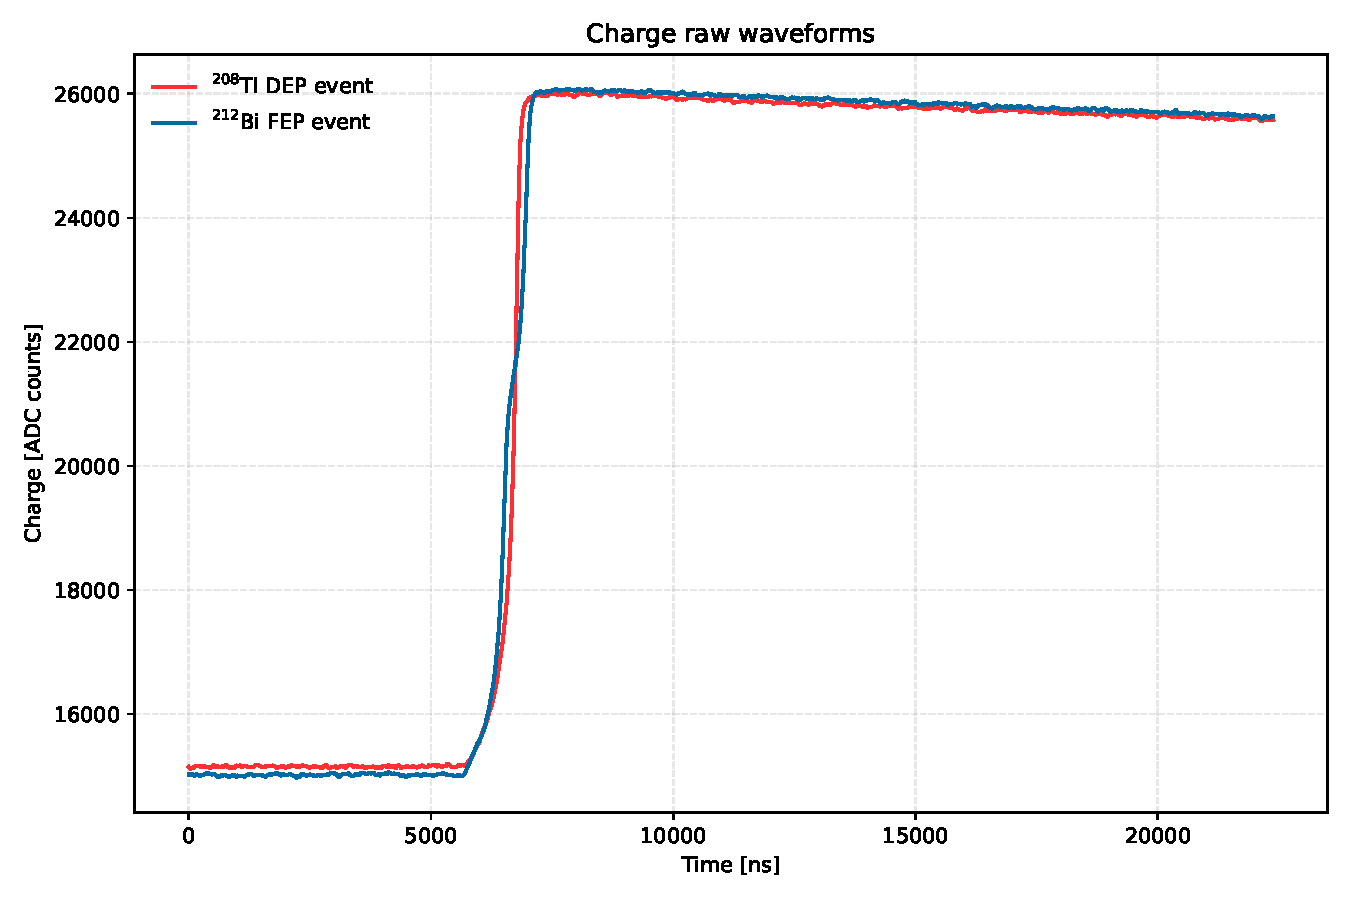
\includegraphics[width=\textwidth]{plots/wfCleaning/raw_wf.pdf}
        \caption{Raw charge waveforms.}
        \label{fig:a-raw-wf}
    \end{subfigure}
    \hfill % Crea uno spazio orizzontale tra le due figure affiancate
    % --- Seconda figura (b) ---
    \begin{subfigure}[H]{0.5\textwidth}
        \centering
        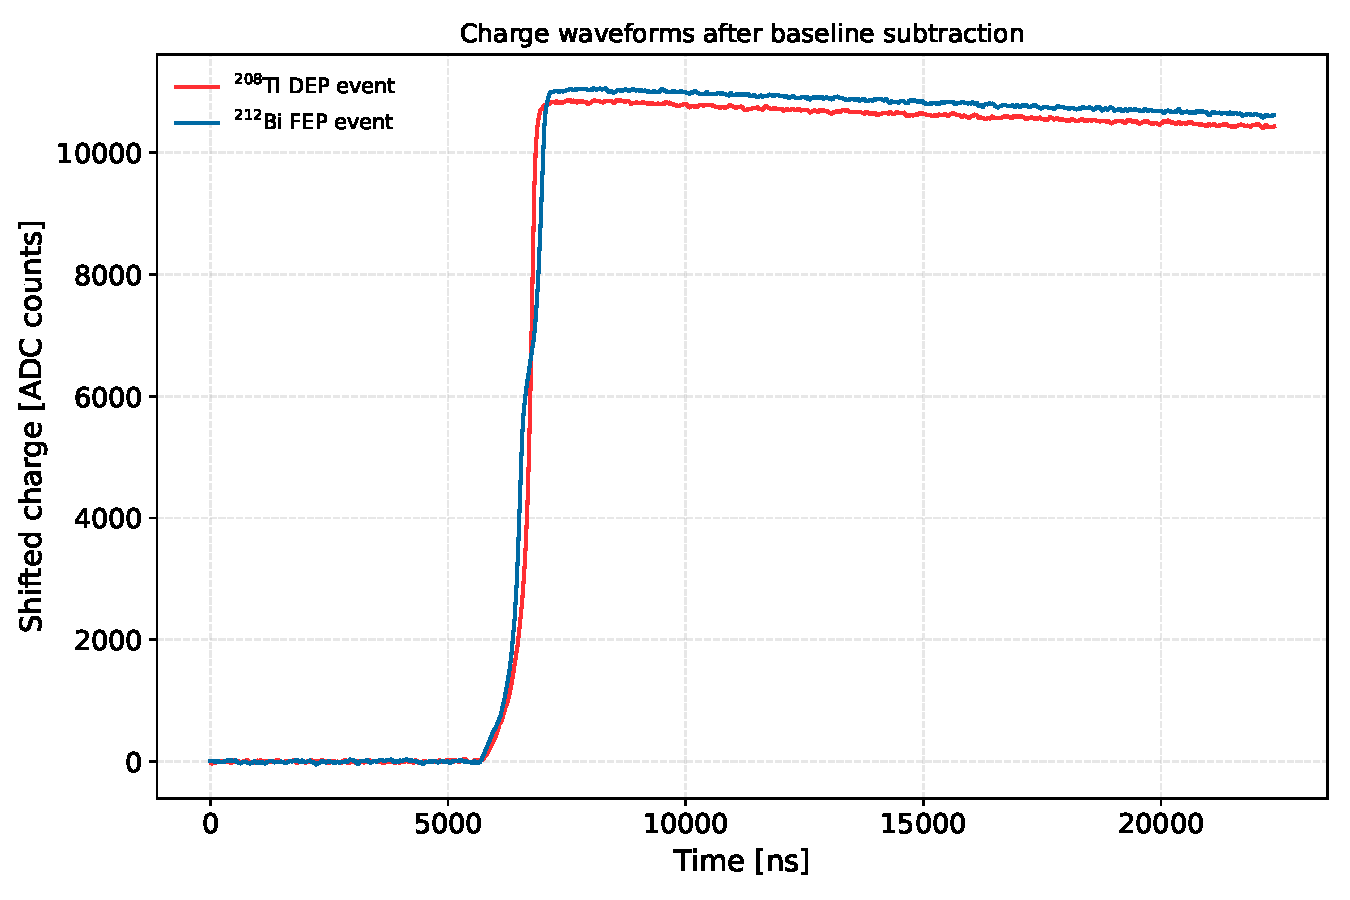
\includegraphics[width=\textwidth]{plots/wfCleaning/baseline_subtracted_wf.pdf}
        \caption{Charge waveforms after baseline subtraction.}
        \label{fig:b-baseline}
    \end{subfigure}
    
    \vspace{0.5cm} % Spazio verticale tra la prima e la seconda riga
    
    % --- Terza figura (c) ---
    \begin{subfigure}[H]{0.48\textwidth}
        \centering
        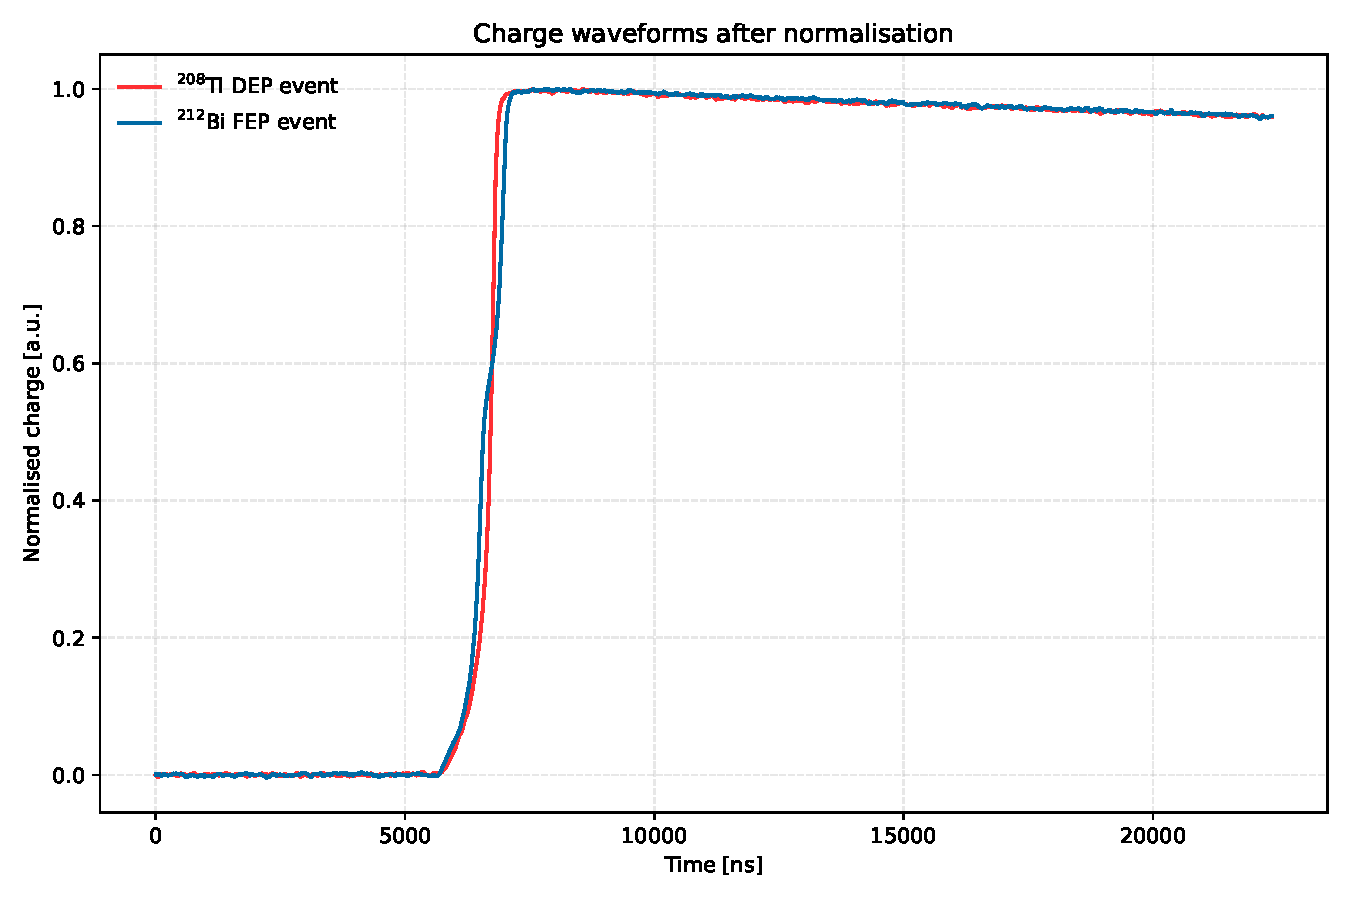
\includegraphics[width=\textwidth]{plots/wfCleaning/normalised_wf.pdf}
        \caption{Charge waveforms after normalisation.}
        \label{fig:c-normalised}
    \end{subfigure}
    \hfill
    % --- Quarta figura (d) ---
    \begin{subfigure}[H]{0.48\textwidth}
        \centering
        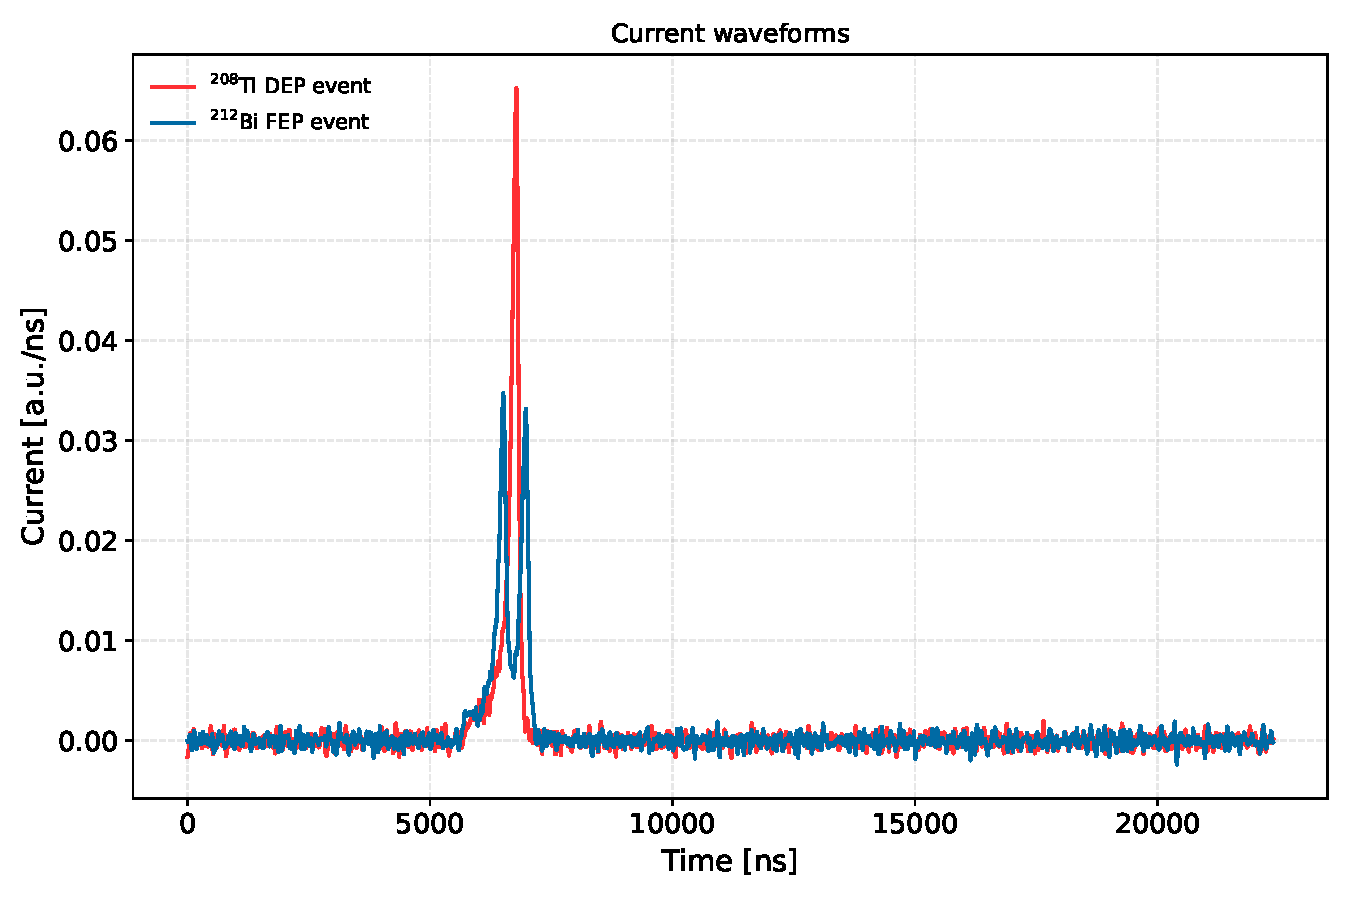
\includegraphics[width=\textwidth]{plots/wfCleaning/current_wf.pdf}
        \caption{Current waveforms btained with time derivative.}
        \label{fig:d-aligned}
    \end{subfigure}

        % --- Quinta figura (e) ---
    \begin{subfigure}[H]{0.48\textwidth}
        \centering
        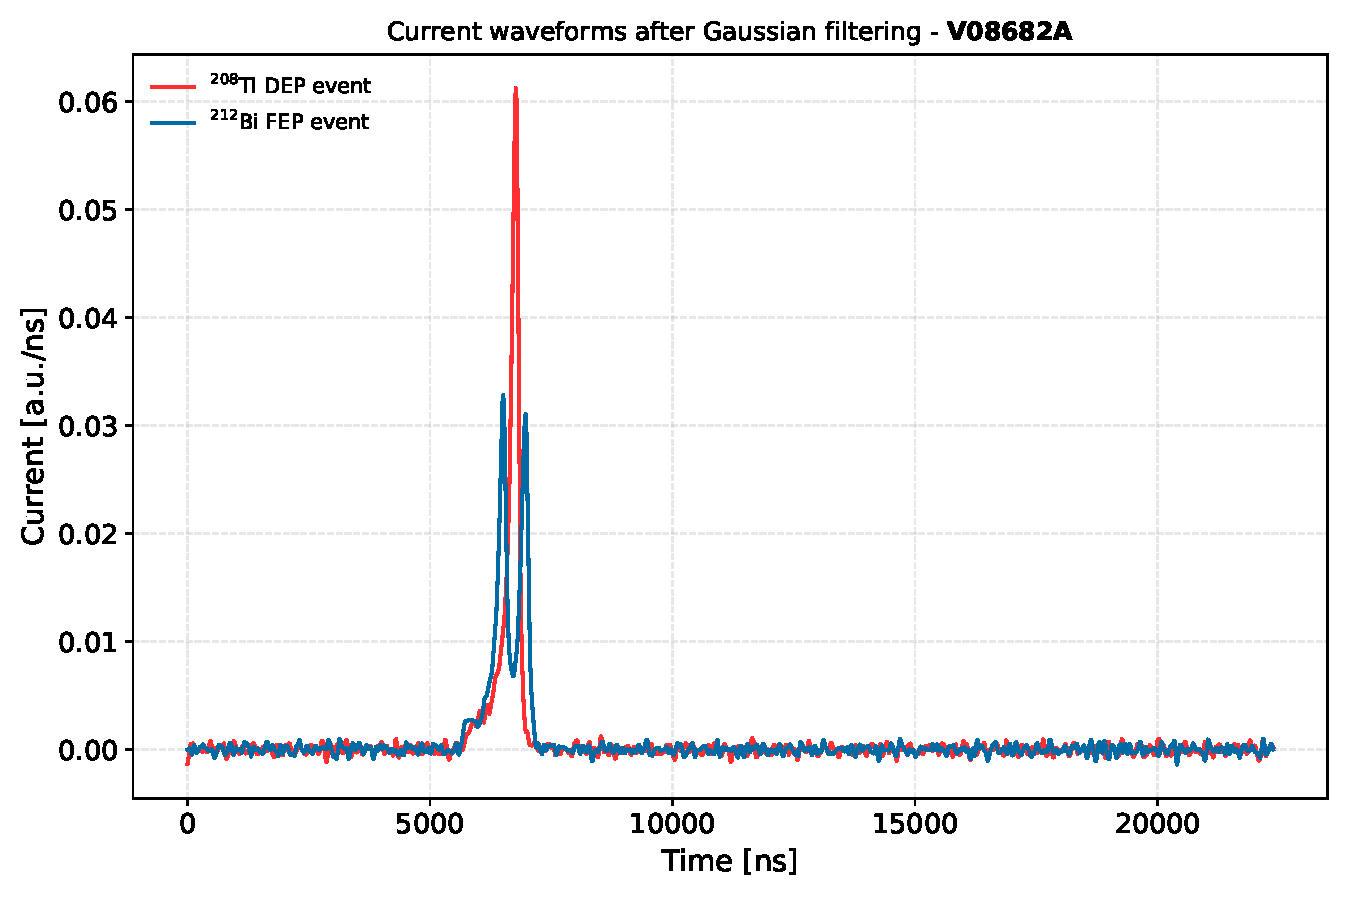
\includegraphics[width=\textwidth]{plots/wfCleaning/current_filtered_wf.pdf}
        \caption{Current waveforms after butterworth filtering.}
        \label{fig:e-trimmed}
    \end{subfigure}
    \hfill
    % --- Sestaa figura (f) ---
    \begin{subfigure}[H]{0.48\textwidth}
        \centering
        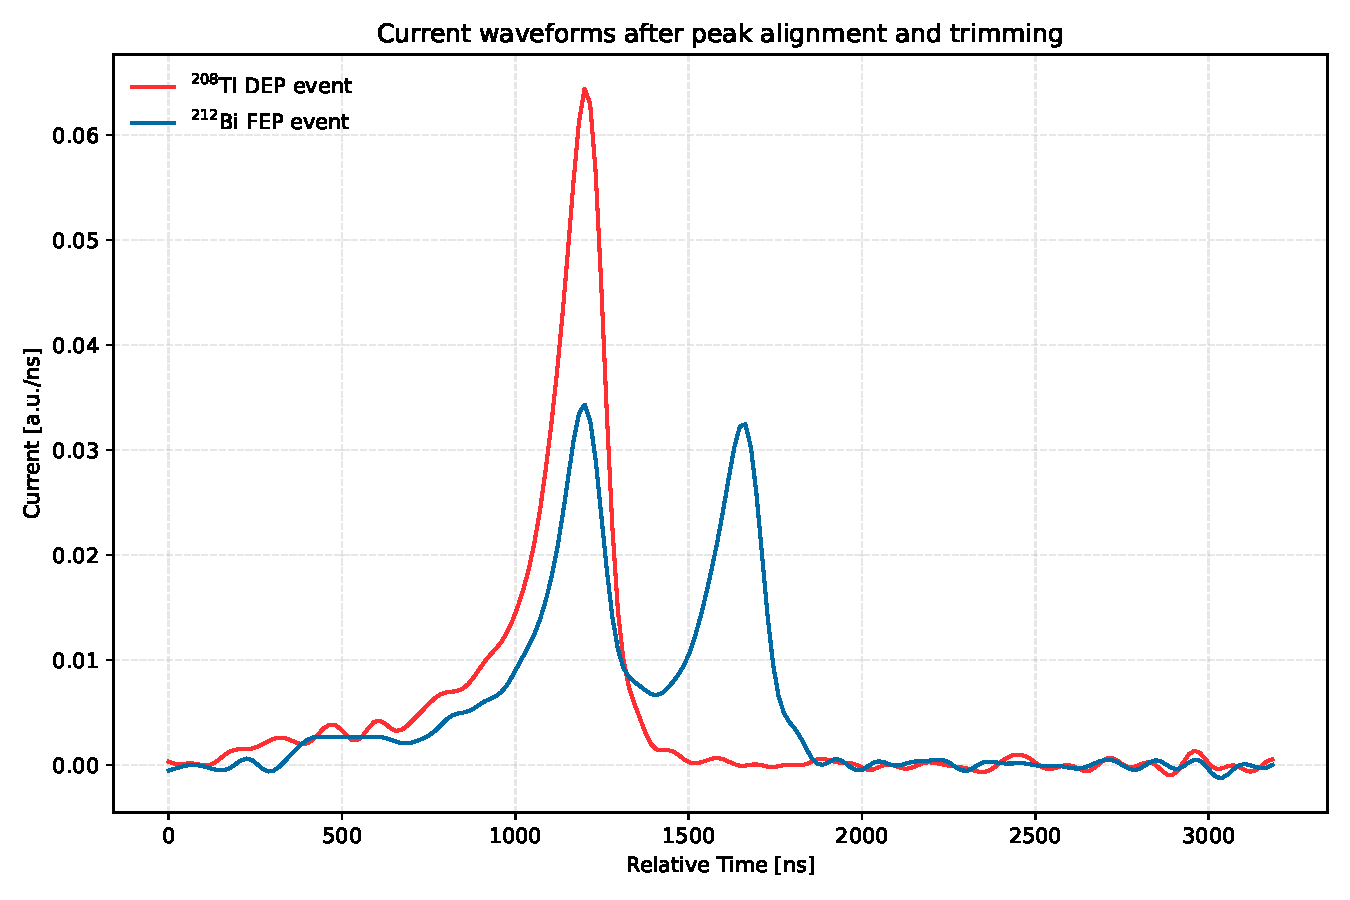
\includegraphics[width=\textwidth]{plots/wfCleaning/current_aligned_filtered_wf.pdf}
        \caption{Current waveforms after peak alignement.}
        \label{fig:f-current}
    \end{subfigure}
    
    % --- Didascalia principale ---
    \caption{Illustration of the workflow of the data processing for two types of waveforms taken from run \textit{r000} of period \textit{p03}: the red one is a typical \ac{MSE} waveform with a non-trivial structure while the blue one is a ordinary \ac{SSE} waveform. A detailed description of the process is given in the text.}
    \label{fig:data-cleaning}
\end{figure}

\newpage
\section{Variational Autoencoder}
\label{sec:VAE}
\ac{SSE} and \ac{MSE} selection is performed through the following procedure. First a gasussian fit is performed onto the \ac{DEP} of ${}^{208}$Tl and the \ac{FEP} of ${}^{212}$Bi via the function of Eq. \ref{eq:fitted-gaussian}
\begin{equation}
    \label{eq:fitted-gaussian}
    f(x) = A \cdot \frac{1}{\sqrt{2 \pi \sigma^2}} \cdot \exp\left(-\frac{(x - \mu)^2}{2\sigma^2}\right) + B
\end{equation}
where $A$ is the total number of events under the peak, i.e. the peak area obtained by integrating the background-subtracted Gaussian componente, $\mu$ is the mean value, $\sigma$ is the standard deviation and $B$ is the background. The results of the fit are reported in Tab. \ref{tab:gaussianfit_parameters}. 
\begin{figure}[H]
    \centering
    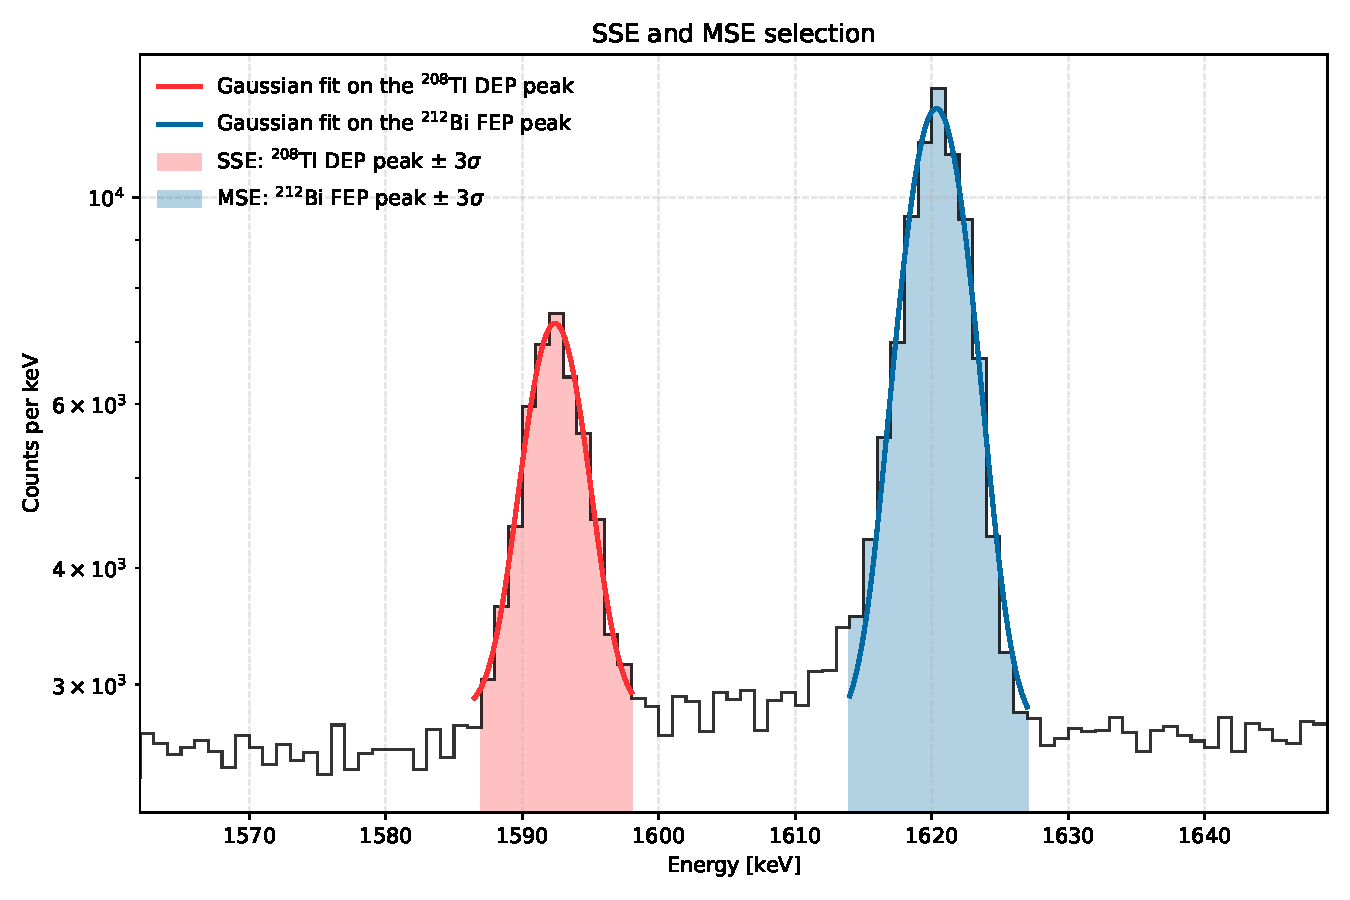
\includegraphics[width=0.8\textwidth]{plots/sse_mse_selection_3sigma.pdf}
    \caption{Events selection for \ac{SSE} and \ac{MSE}. A detailed description of the procedure is given in the text.}
    \label{fig:sse_mse_cut}
\end{figure} 

\begin{table}[H]
  \centering
  \begin{tabular}{ccccc}
    \toprule
    Peak & Amplitude [counts] & $\mu$ [keV] & $\sigma$ [keV] & Background [counts/keV] \\
    \midrule
    ${}^{208}\text{Tl}$ & $(2.4 \pm 0.2) \times 10^{4}$ & $1592.40 \pm 0.06$ & $2.1 \pm 0.1$ & $(2.8 \pm 0.2) \times 10^{3}$ \\
    ${}^{212}\text{Bi}$ & $(5.7 \pm 0.7) \times 10^{4}$ & $1620.34 \pm 0.08$ & $2.3 \pm 0.2$ & $(2.7 \pm 0.6) \times 10^{3}$ \\
    \bottomrule
  \end{tabular}
  \caption{Gaussian fit parameters for the ${}^{208}\text{Tl}$ \ac{DEP} and ${}^{212}\text{Bi}$ \ac{FEP}.}
  \label{tab:gaussianfit_parameters}
\end{table}
Secondly, the selcetion needs to consider only a part of the events under the peaks. A standard 3$\sigma$ cut around the mean value of each peak is shown in Fig. \ref{fig:sse_mse_cut} in light red and light blue for ${}^{208}$Tl and ${}^{212}$Bi respectively. Nevertheless it is clear thet those peaks are not purely \ac{SSE} or \ac{MSE} but rather a mixture of both since the continuum background is present in the whole energy spectrum. A cut window within a different number of sigmas would lead to different results in terms of \ac{SSE} and \ac{MSE} purity. In order to get an idea of such fractions we can consider, for different $\sigma$ cuts, the ratio between the total number of events under the peak and background part of them; these are parametrised respectively by the $A$ and $B$ paramters of Eq. \ref{eq:fitted-gaussian}.
Table~\ref{tab:purity} shows that the \ac{DEP} sample exhibits a systematically lower purity than the \ac{FEP} sample across the considered window widths. This is expected, since the \ac{FEP} peak amplitude is substantially bigger than the \ac{DEP} one while the underlying background level is comparable (see Tab.~\ref{tab:gaussianfit_parameters}), resulting in a more favourable peak-to-background ratio for the \ac{FEP} selection. This consideration is particularly relevant when we need to consider the performance of the deep learning classifier, since it is trained in a supervised mode: mislabelled events (i.e. continuum events wronlgy assigned to the \ac{SSE} or \ac{MSE} class) directly enter the loss function computation, injecting label noise that biases both the training process and the resulting final performance.

\begin{table}[H]
\centering
\begin{minipage}{0.48\textwidth}
\centering
\begin{tabular}{cccc}
\toprule
$\sigma$ & peak counts & background counts & purity \\
\midrule
0.5 & 9117  & 5919  & 60.6\% \\
1.0 & 16255 & 11838 & 57.9\% \\
1.5 & 20629 & 17758 & 53.7\% \\
2.0 & 22727 & 23677 & 49.0\% \\
2.5 & 23514 & 29596 & 44.3\% \\
3.0 & 23746 & 35515 & 40.1\% \\
\bottomrule
\end{tabular}
\caption{\ac{DEP} sample}
\label{tab:purity_sse}
\end{minipage}
\hfill
\begin{minipage}{0.48\textwidth}
\centering
\begin{tabular}{cccc}
\toprule
$\sigma$ & peak counts & background counts & purity \\
\midrule
0.5 & 21873 & 6229  & 77.8\% \\
1.0 & 38996 & 12457 & 75.8\% \\
1.5 & 49489 & 18686 & 72.6\% \\
2.0 & 54523 & 24914 & 68.6\% \\
2.5 & 56412 & 31143 & 64.4\% \\
3.0 & 56968 & 37372 & 60.4\% \\
\bottomrule
\end{tabular}
\caption{\ac{FEP} sample}
\label{tab:purity_mse}
\end{minipage}
\caption{Peak counts, background counts and purity for a different number of sigmas considered in the cut window for the \ac{DEP} and \ac{FEP} samples.}
\label{tab:purity}
\end{table}



% \begin{figure}[H]
%     \centering 
%     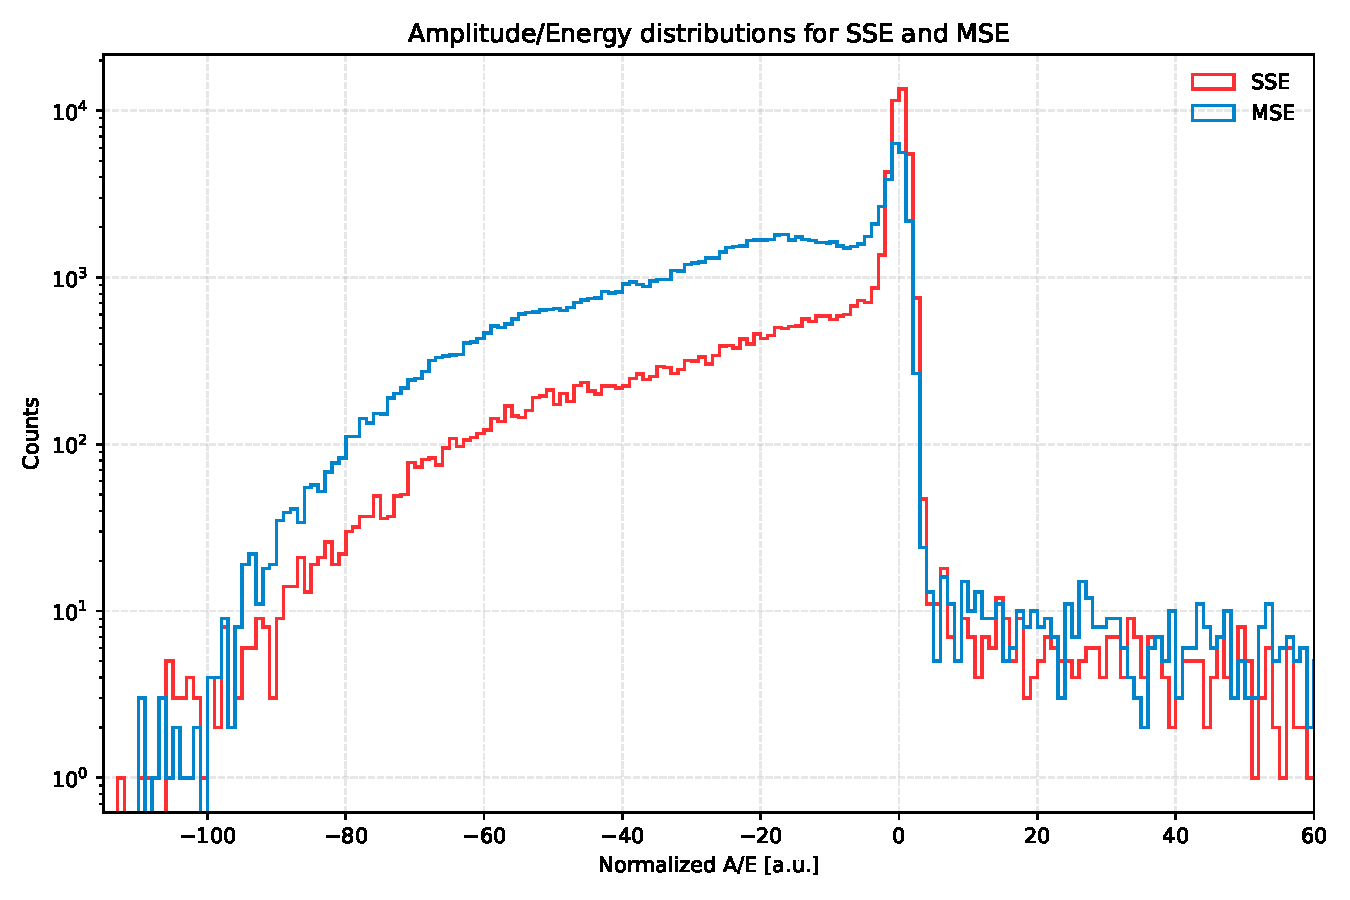
\includegraphics[width=0.7\textwidth]{plots/AoE_sse_vs_sse.pdf}
%     \caption{Distributions of the Amplitude/Energy quantity for SSE and MSE.}
%     \label{fig:AoE-sse_vs_mse}
% \end{figure}

\subsection{Variational Autoencoder architecture}
\label{sec:model-architeture}
\begin{comment}
QUI DEVO DIRE

-COME CREO I TENSORS --> TENSORCREATION.PY

-COME IMPLEMENTO IL VAE

    - encoder\\
    - decoder\\
    - latent space specifications\\
    - costruzione della loss\\
    - training\\ 
    - test\\
    - tutti i test del codice che faccio\\
        * test su beta
        * test su dimensioni dello spazio lentamente
        * eventuale PCA e/o TRAVERSAL
- COME IMPLEMENTO LA CLASSIFICATION\\
    - layers etc\\ 
    - loss\\
    - training \\
    - test \\
\end{comment}

\begin{figure}[H]
    \centering
    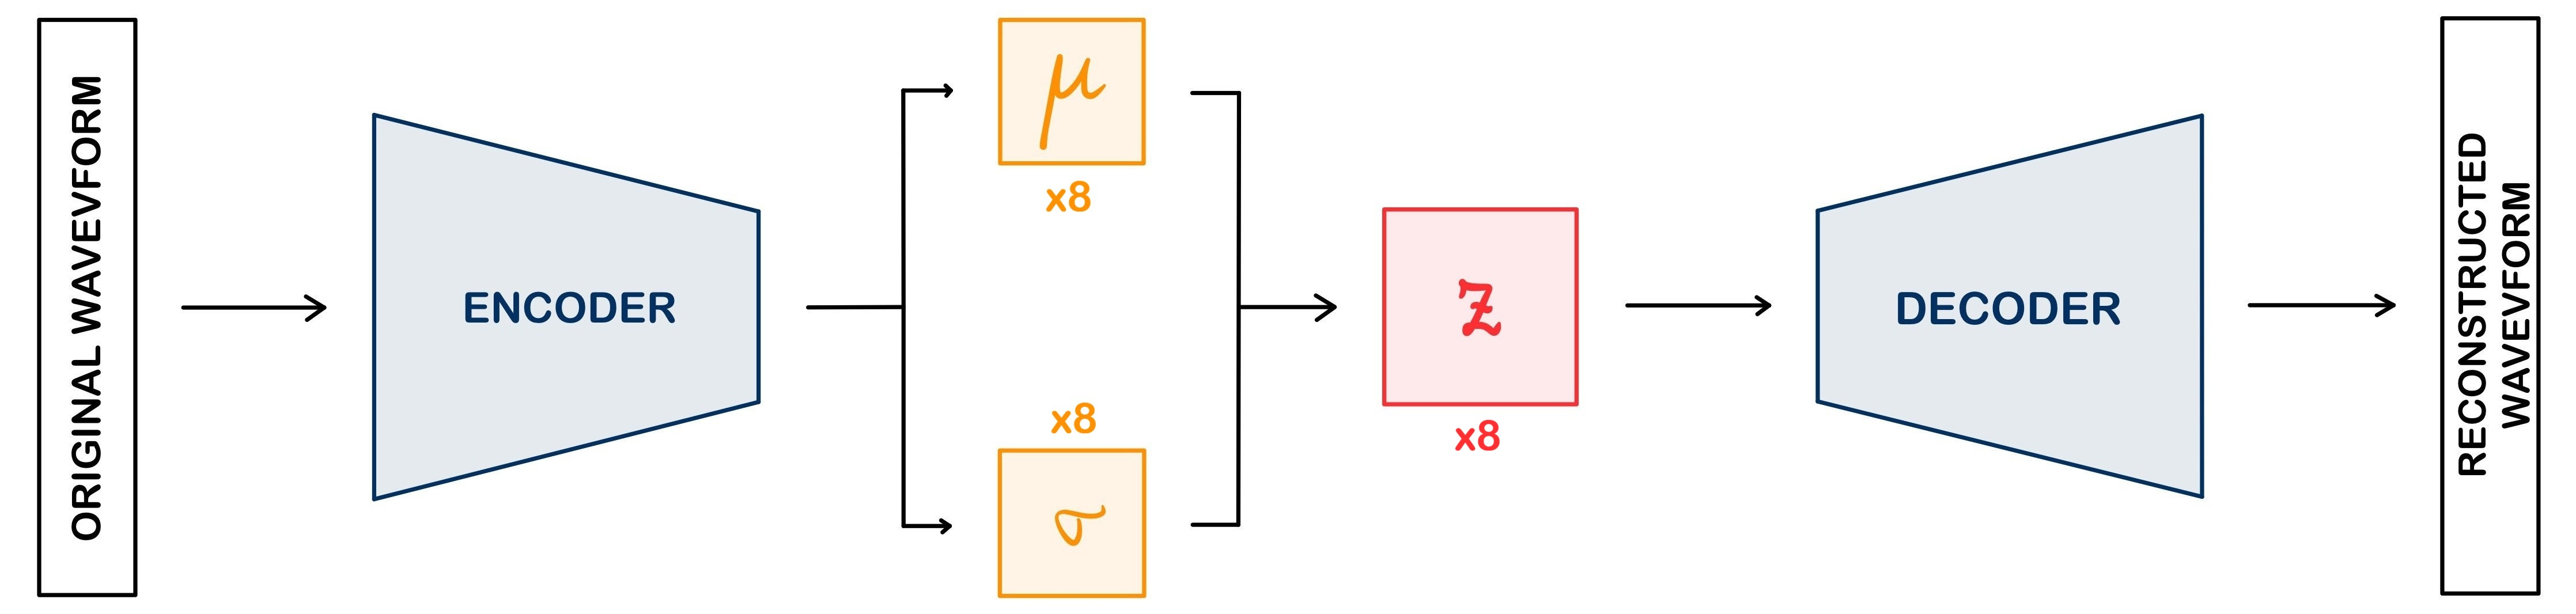
\includegraphics[width=\textwidth]{figures/schemaVAE.jpg}
    \caption{Schematic representation of the $\beta$-VAE architecture. The encoder network maps the input waveform to a latent space characterized by a mean and variance, from which a latent vector is sampled. The decoder reconstructs the waveform from this latent representation. The loss function combines reconstruction loss and KL divergence, weighted by the hyperparameter $\beta$.}
    \label{fig:vae-architecture}
\end{figure}


\subsection{Variational Autoencoder results}
QUI DEVO SPERARE CHE IL ML FUNZIONI MEGLIO DELL'AvsE






\newpage
\section{Self-organising map}
A \ac{SOM} is an unsupervised machine learning tecnique used to produce low-dimensionality representation of a higher-dimensionality dataset preserving topological structures of data that distinguish different types of said data. Specifically, a \ac{SOM} is a type of artificial neural network trained using competitive learning rather than error-correction learning. The goal in these auto-organised learning maps is to train different parts of the \ac{SOM} to reply to different input patterns: this specific design has been formulated in the 1980s by Teuvo Kohonen on the basis of how the human brain manages different information in different parts of the cerebral cortex.

Starting from weights vectors initialised to casual or very small numbers, the algorithm exploits competitive learning: when a new training sample is received by the network, the a distance metric is computed from all the weights vectors. The most alike weights vector, named \ac{BMU} and all the neurons near to ir in the \ac{SOM} net are brought closer with one another and weights are updated.